\documentclass[12pt, a4paper]{article}
\usepackage{graphicx}
\graphicspath{{./images/}}
\usepackage{listings}
\usepackage[hidelinks]{hyperref}
\usepackage{color}

\definecolor{dkgreen}{rgb}{0,0.6,0}
\definecolor{gray}{rgb}{0.5,0.5,0.5}
\definecolor{mauve}{rgb}{0.58,0,0.82}

\lstset{frame=tb,
  language=Python,
  aboveskip=3mm,
  belowskip=3mm,
  showstringspaces=false,
  columns=flexible,
  basicstyle={\small\ttfamily},
  numbers=none,
  numberstyle=\tiny\color{gray},
  keywordstyle=\color{blue},
  commentstyle=\color{dkgreen},
  stringstyle=\color{mauve},
  breaklines=true,
  breakatwhitespace=true,
  tabsize=3
}
\title{Aufbau eines drahtlosen Netzwerks}
\author{Benedikt Viebahn s0565139}
\begin{document}
\maketitle
\tableofcontents 
\newpage
\section{Einleitung}
Im Rahmen der Veranstaltung Technik Mobiler Systeme haben wir 
ein drahtloses Netzwerk mit Raspberry Pis aufgebaut. Die Aufgaben bestanden 
darin, den Raspberry Pi mit einem Microcontroller auszustatten, 
und ein Protokoll zu implementieren auf das wir uns vorher geeinigt hatten,
und über das wir andere Netzwerktteilnehmer
finden und mit ihnen kommunizieren können. 

\section{Einrichtung}
Damit MCU und Raspberry Pi miteinander kommunizieren können 
müssen diese sowohl Hardware-, als auch Softwareseitig 
richtig konfiguriert werden.
Die von uns verwendete MCU benötigt eine Verbindung zur Stromquelle,
zu Ground, und jeweils eine Verbindung um Daten zu empfangen und zu senden.
Die Pins müssen wie folgt miteinander verbunden werden (siehe Figure 1-3):
\begin{center}
    \begin{tabular}{|c|c|}
        \hline
        Raspberry Pi & MCU \\ [0.5ex]
        \hline\hline
        Ground & GND \\
        \hline
        3.3 VDC Power & VIN \\
        \hline
        GPIO 15 TxD (UART) & RX \\
        \hline
        GPIO 16 RxD (UART) & TX \\
        \hline
    \end{tabular}
\end{center}

\newpage
\begin{figure}[ht!]
    \centering
    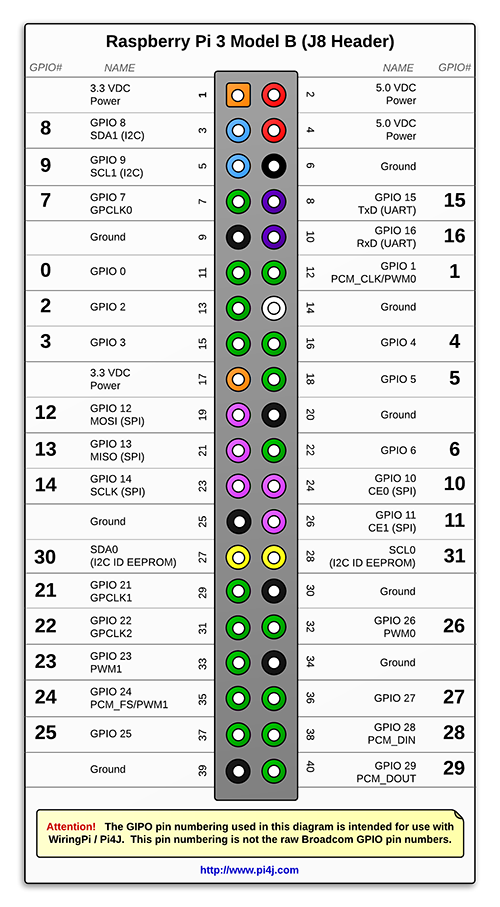
\includegraphics[width=300pt]{j8header}
    \caption{Raspberry Pi Anschlüsse}
\end{figure}
\begin{figure}[ht!]
    \centering
    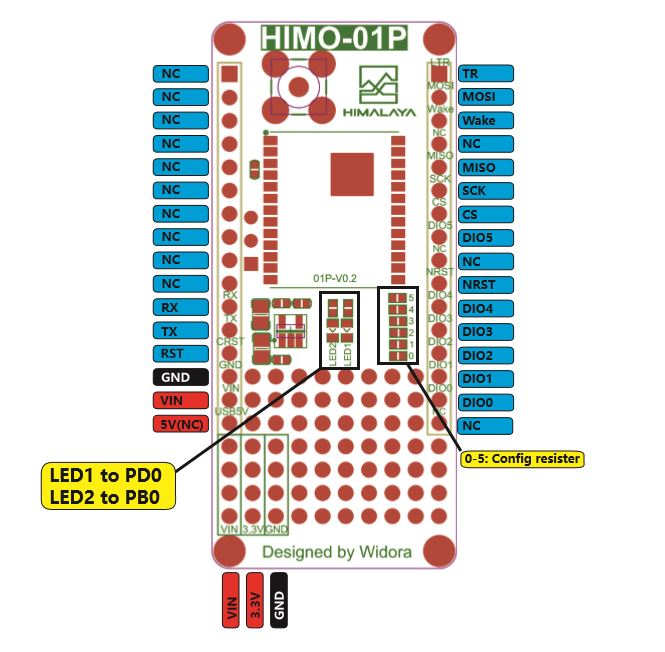
\includegraphics[width=300pt]{mcu}
    \caption{MCU Anschlüsse}
\end{figure}
\begin{figure}[ht!]
    \centering
    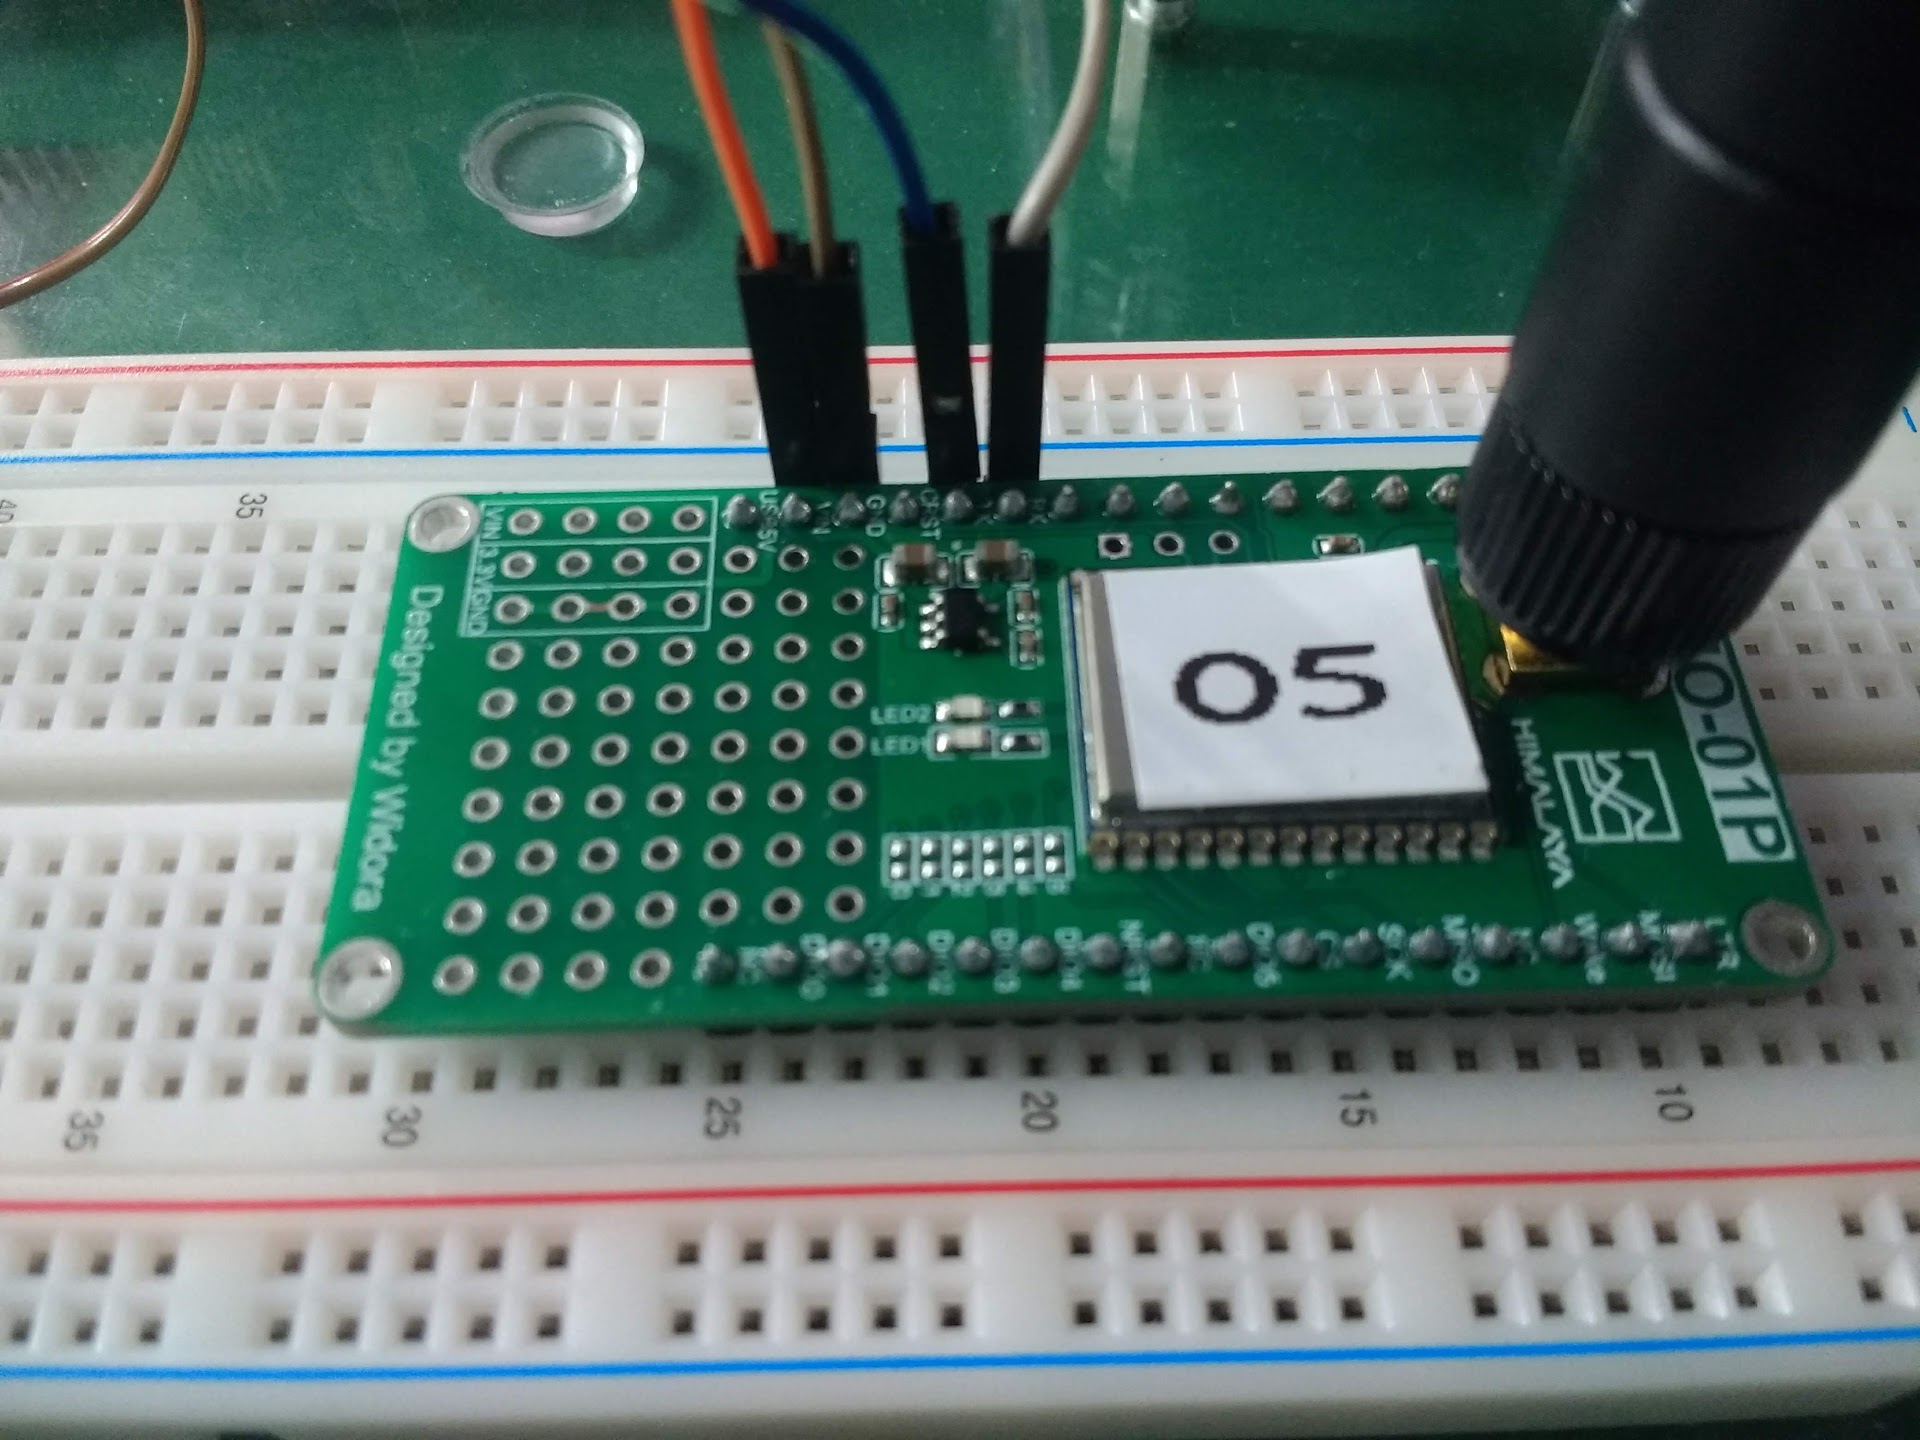
\includegraphics[width=300pt]{mcu_photo}
    \caption{MCU fertig verbunden}
\end{figure}
\clearpage
Nachdem die Hardware richtig verbunden ist muss eventuell der Serial Port 
in den Einstellungen des Raspberry Pis unter Interfaces freigegeben werden.
Mit dem Programm \textit{cutecom} kann getestet werden ob die Kommunikation
funktioniert. Das Programm sollte so konfiguriert werden:
\begin{center}
    \begin{tabular}{|c|c|}
        \hline
        Konfiguration & Wert \\ [0.5ex]
        \hline\hline
        Baudrate & 115200 Bits \\
        \hline
        Parity Bit & NONE \\
        \hline
        Stop bits & 1 \\
        \hline
        Data bits & 8 \\
        \hline
    \end{tabular}
\end{center}
\section{Kommunikation mit AT Befehlen}
Nun kann mit AT Befehlen getestet werden ob die Verbindung funktioniert.
Wenn \textbf{AT\textbackslash{}r\textbackslash{}n}
\textbf{AT,OK\textbackslash{}r\textbackslash{}n} zurück liefert funktioniert
die Komminikation.
Mit \textbf{AT+ADDR=XXXX\textbackslash{}r\textbackslash{}n} kann die eigene
Adresse festgelegt werden. XXXX ist dabei die Adresse und kann im Bereich von
0000 bis FFFF liegen, wobei FFFF die Broadcastadresse ist. Nachrichten an diese
Adresse werden von allen empfangen.
Um Daten zu senden muss zunächst mit \textbf{AT+DEST=XXXX\textbackslash{}r\textbackslash{}n}
die Zieladresse festgelegt werden. Das Modul antwortet darauf wieder mit \textbf{AT,OK\textbackslash{}r\textbackslash{}n}.
Dannach wird mit 
\textbf{AT+SEND=XX\textbackslash{}r\textbackslash{}n} die Größe der zu sendenden
Daten angegeben. Dabei sollte beachtet werden, dass die maximale Länge 25 Byte 
beträgt. Daten die die festgelegte Länge überschreiten werden verworfen.
Nachdem das Modul mit \textbf{AT,OK\textbackslash{}r\textbackslash{}n} antwortet,
können nun Daten übertragen werden. Dabei antwortet das Modul erst mit 
\textbf{AT,SENDING\textbackslash{}r\textbackslash{}n} um mitzuteilen dass es sich im 
Sendezustand befindet, und nach erfolgreicher Übertragung mit
\textbf{AT,SENDED\textbackslash{}r\textbackslash{}n}.

\section{Protokoll}
Zur Entdeckung der Netzwerkteilnehmer haben wir uns auf folgendes 
Network Discovery Protokoll geeinigt:
Jeder Teilnehmer sendet mit zufälligen Abständen zwischen 30 und 60 Sekunden
eine Nachricht mit dem Inhalt \textbf{RTI} an die Broadcastadresse \textbf{FFFF}.
Jeder der diese Nachricht empfängt kann die Senderadresse speichern und 
weiß nun dass sie existiert und dass sie erreicht werden kann.

\section{Implementierung}
Das Script wurde in Python geschrieben und funktioniert wie folgt:
Um auf die serielle Schnittstelle zuzugreifen wird das package \textit{serial}
verwendet.
\begin{lstlisting}
    import serial
    ser = serial.Serial(
        port='/dev/ttyS0',
        baudrate=115200,
        parity=serial.PARITY_NONE,
        stopbits=serial.STOPBITS_ONE,
        bytesize=serial.EIGHTBITS
    )
    ser.isOpen()
\end{lstlisting} 
Als nächstes legen wir unsere Adresse fest. Diese wird dem Programm beim
Aufruf als Argument übergeben.
\begin{lstlisting}
    ser.write("AT+ADDR=" + sys.argv[1] + "\r\n")
\end{lstlisting}
Die momentan ausgewählte Zieladresse, die empfangenen Nachrichten und
die bekannten Adressen werden gespeichert und immer aktuell gehalten.
Außerdem wird gespeichert ob gerade auf eine \textbf{AT,OK} Nachricht gewartet wird,
und ob eine empfangen wurde. Dadurch wird gewährleistet, dass Nachrichten 
erst gesendet werden nachdem alle vorher gesendeten Nachrichten angekommen sind.
Das Programm nutzt drei Threads (+ main thread): \\
\textbf{receive:} 
Daten werden von der seriellen Schnittstelle empfangen und in einem Array 
für die spätere Verarbeitung gespeichert. \\
\textbf{processReceived:} 
Die empfangenen Nachrichten werden in der Reihenfolge in der sie 
empfangen wurden bearbeitet. Beim Empfangen einer \textbf{AT,OK}
Nachricht wird ein globales Boolean \textit{ok} auf \textit{True} gesetzt.
Ein anderer Thread der zuvor etwas gesendet hat und auf \textbf{AT,OK}
wartet kann jetzt weiter machen und setzt \textit{ok} und \textit{waitingForOk}
auf \textit{False} wodurch anderen Teilen des Programms signalisiert 
wird, dass neue Nachrichten gesendet werden können.
Beim Empfangen einer Nachricht mit dem Inhalt \textbf{RTI} wird die Adresse
ausgelesen und gespeichert falls sie noch nicht bekannt ist. \\
\textbf{sendRTI:}
Dieser Thread sendet RTI Nachrichten und schläft dann 30-60 Sekunden. \\
Im Main Thread werden Benutzereingaben ausgewertet. Mit \textit{exit} kann das
Programm beendet werden. Mit \textit{printtable} werden alle bekannten Adressen 
ausgegeben. Mit \textit{send;ADDR;MESSAGE} wird eine Nachricht gesendet.

\section{Quellen}
\hyperlink{http://www.pi4j.com}{www.pi4j.com} \\
\hyperlink{https://www.widora.io/zh/ting_at}{www.widora.io}
\end{document}